\documentclass{standalone}
\usepackage{tikz}
\begin{document}
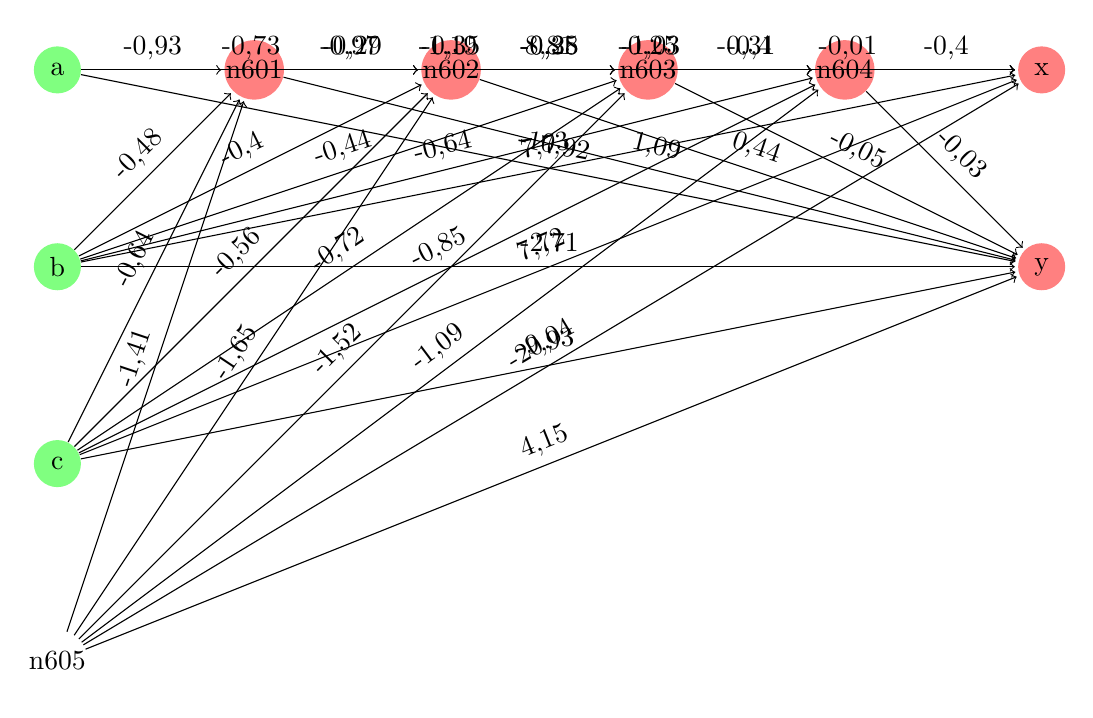
\begin{tikzpicture}[shorten >=1pt,->,draw=black!,node distance=2.5cm]
\tikzstyle{neuron}=[circle,fill=black!25,minimum size=17pt,inner sep=0pt]
\tikzstyle{constant}=[neuron, fill=white!50];
\tikzstyle{sigmoid}=[neuron, fill=red!50];
\tikzstyle{identity}=[neuron, fill=green!50];
\node [identity] (a) {a};
\node [identity,below of=a] (b) {b};
\node [identity,below of=b] (c) {c};
\node [constant,below of=c] (n605) {n605};
\node [sigmoid,right of=a] (n601) {n601};
\node [sigmoid,right of=n601] (n602) {n602};
\node [sigmoid,right of=n602] (n603) {n603};
\node [sigmoid,right of=n603] (n604) {n604};
\node [sigmoid,right of=n604] (x) {x};
\node [sigmoid,below of=x] (y) {y};
\path[every node/.style={sloped,anchor=south,auto=false}]
(n602) edge node {-0,4} (x)
(n602) edge node {0,44} (y)
(n602) edge node {-0,35} (n603)
(n602) edge node {-0,25} (n604)
(n601) edge node {-1,03} (x)
(n601) edge node {1,09} (y)
(n601) edge node {-0,29} (n602)
(n601) edge node {-0,35} (n603)
(n601) edge node {-0,28} (n604)
(n604) edge node {-0,4} (x)
(n604) edge node {-0,03} (y)
(n603) edge node {-0,01} (x)
(n603) edge node {-0,05} (y)
(n603) edge node {-0,31} (n604)
(n605) edge node {-20,04} (x)
(n605) edge node {4,15} (y)
(n605) edge node {-1,41} (n601)
(n605) edge node {-1,65} (n602)
(n605) edge node {-1,52} (n603)
(n605) edge node {-1,09} (n604)
(c) edge node {-0,64} (n601)
(c) edge node {-9,93} (y)
(c) edge node {7,72} (x)
(c) edge node {-0,85} (n604)
(c) edge node {-0,72} (n603)
(c) edge node {-0,56} (n602)
(b) edge node {-2,71} (y)
(b) edge node {7,73} (x)
(b) edge node {-0,64} (n604)
(b) edge node {-0,44} (n603)
(b) edge node {-0,4} (n602)
(b) edge node {-0,48} (n601)
(a) edge node {8,81} (x)
(a) edge node {-0,97} (n603)
(a) edge node {-0,73} (n602)
(a) edge node {-0,93} (n601)
(a) edge node {-10,92} (y)
(a) edge node {-1,19} (n604)
;\end{tikzpicture}
\end{document}